\chapter{Introduction}


In this section, an introduction to machine learning and graph neural networks is provided. 
This is followed by a discussion about attribution based explainable machine learning methods 
in a game theoretical framework. Subsequently, molecular representation and the chemical 
problem are addressed.


\section{Machine learning}


Machine learning algorithms require a feature matrix $\mathbf{X} \in \mathbb{R}^{N \times p}$
where each row represents a sample and each column relates to an attribute. 
Supervised ML additionally requires a target vector $\pmb{y} \in \mathbb{R}^N$
representing another feature with a value for each sample. Then, the goal of an ML method is 
to construct a function $f$, based on parameters $\pmb{\theta}$, that can accurately 
predict the outcome variable $\pmb{y}$ of the training data $\pmb{X}$ and can 
generalize to new data.\cite{hastie2009elements} After obtaining the predicted 
values $\hat{\pmb{Y}} = f\left(\pmb{X}; \pmb{\theta}\right)$, they are compared 
to the true values $\pmb{y}$ (also called labels)
in order to determine how good the model is, which introduces the concept of loss functions $\mathcal{L}$.
Different loss functions exists for different kind of problems.\cite{wang2020comprehensive}
A commonly used loss function is the mean squared error (MSE) (\cref{eq:mse})
which averages the squared difference between the predicted value and true label.
Furthermore, optimizing the loss function with respect to the learning function
parameters produces the best model with the given architecture.\cite{hastie2009elements}


\begin{equation}
	\label{eq:mse}
	\text{MSE}\big(\pmb{y}, \pmb{X}\big) = \frac{1}{N}  \big[\pmb{y} - f(\mathbf{X})\big]^T[\pmb{y} - f(\mathbf{X})\big]
\end{equation}


One of the simplest functions $f\left(\mathbf{X}; \pmb{\theta}\right) = \mathbf{X}\pmb{\theta}$
is a linear combination of the features, where $\pmb{\theta} \in \mathbb{R}^p$
is the vector of coefficients. This model, known as linear regression, is commonly
used in statistical modeling.\cite{kutner2005applied} Although the linear model is
very interpretable, the linearity constraint is too strict which limits its
applicability. Therefore, more complicated ML algorithms were developed which are
able to obtain improved performance on complicated data with respect to linear
regression by allowing non-linear relationships.\cite{deng2012mnist} However,
they pay a price in terms of interpretability.\cite{fan2021interpretability}


\section{Neural networks}


Neural networks (NN) are a class of machine learning algorithms which are able to
approximate complicated non-linear function, inspired by the human brain.
\cite{cybenko1989approximation, rosenblatt1962principles} Although a NN is a strong
simplification of the human brain, the concept of neuron signal transit is used 
as a basic building block.\cite{wang2017origin} This signal transmission
takes place between units in a neural network. Then, different architectures
can be used to connect different units. Rosenblatt proposed a weighted sum 
of the inputs followed by a non-linear activation function.\cite{rosenblatt1962principles}
This neural network is, however, still a linear function due to its inability 
to learn non-linear functions. A solution to this limitation is stacking multiple 
perceptrons after each other, resulting in a multi layer perceptron (MLP).
The multi layer perceptron (MLP) is a basic architecture that is frequently 
utilized in other, more complicated neural networks.\cite{almeida2020multilayer}
In an MLP (\cref{fig:mlp_structure}) three parts can be distinguished: an input layer,
one or more hidden layers and an output layer.


\begin{figure}[h]
	\centering
	\includegraphics[scale=1.5]{mlp.png}
	\caption{General structure of a multi layer perceptron (MLP) consisting of an input layer,
		one or multiple hidden layers and an output layer. The symbol separating two layers denote that
		all neurons between these two layers are connected.}
	\label{fig:mlp_structure}
\end{figure}


The values of the input layer are equal to the given feature matrix
$\pmb{X}$. Let $n^{(1)}$ denote the number of units in the first hidden layer.
Then taking $n^{(1)}$ different linear combinations of the input layer followed by
a non-linear activation function $\sigma$ results in the values of this first hidden
layer. Generally, the values $\pmb{H}^{(l)} \in \mathbb{R}^{N \times n^{(l)}}$ of layer
$l$ are given by


\begin{equation}
	\pmb{H}^{(l)} =  \sigma^{(l)} \left(\pmb{H}^{(l-1)}\pmb{\Theta}^{(l-1)} \right),
\end{equation}


where $\pmb{\Theta}^{(l-1)} \in \mathbb{R}^{n^{(l-1)} \times n^{(l)}}$ is the weights matrix
of layer $l - 1$, with $n^{(l-1)}$ and $n^{(l)}$ the number of units in layers
$l-1$ and $l$ respectively and $\pmb{H}^{(0)} = \pmb{X}$. Popular activation
functions are listed in \cref{tab:activation_functions}.

\begin{table}[h]
	\caption{Popular activation functions used in multi layer perceptrons.}
	\label{tab:activation_functions}
	\begin{center}
		\begin{tabular}{c|c}
			\toprule
			Sigmoid(x) = $ \frac{1}{1 + e^{-x}}$                 &
			Softmax(x) = $\frac{e^x}{\sum_{i=1}^{n_L} e^{x_i}}$                                                           \\
			\midrule
			ReLU(x)\cite{glorot2011deep} = $\begin{cases}
					                                x & \text{if } x > 0 \\
					                                0 & \text{otherwise}
				                                \end{cases}$        &
			LeakyReLU(x)\cite{maas2013rectifier} =  $\begin{cases}
					                                         x        & \text{if } x > 0 \\
					                                         \alpha x & \text{otherwise}
				                                         \end{cases}$
			\\ & with $\alpha \ge 0$
			\\
			\midrule
			SeLU(x)\cite{klambauer2017self} = $\lambda \begin{cases}
					                                           x               & \text{if } x > 0 \\
					                                           \alpha(e^x - 1) & \text{otherwise}
				                                           \end{cases}$
			                                                     &
			Gelu(x)\cite{hendrycks2016gaussian} = $\begin{cases}
					                                       x            & \text{if } x > 0 \\
					                                       x \, \Phi(x) & \text{otherwise}
				                                       \end{cases}$
			\\
            see \citen{klambauer2017self} for values of $\alpha$ and $\lambda$ & with $\Phi(x)$ cumulative standard normal distribution \\
			\bottomrule
		\end{tabular}
	\end{center}
\end{table}

An MLP often does not assess the whole feature matrix at once. Rather, the feature
matrix is split up into many batches. Then, following each batch, the parameters are
updated using an optimization algorithm. Common optimization algorithms in neural networks
are gradient descent and Adam.


\subsection{Gradient descent}


A popular optimization algorithm to optimize the weights $\pmb{\Theta}$ of a neural network is
gradient descent.\cite{ruder2016overview} As the name implies, this algorithm
uses the gradient of the loss function $\mathcal{L}$ to step in the direction of the
steepest decline. The size of this step is determined by the learning rate $\alpha$.

\begin{equation}
	\pmb{\Theta}_{t+1} = \pmb{\Theta}_{t} - \alpha \nabla_{\pmb{\Theta}} \mathcal{L}
\end{equation}

Computation of the gradient can be achieved using the backpropagation algorithm, which
propagates the gradient layer by layer through the network starting at the output.
\cite{lecun1988theoretical} One limitation of gradient descent is the
fixed learning rate that has to be chosen thoughtfully at the start of training.
If the learning rate is too large, the step can pass beyond the minimum. Otherwise,
if the learning rate is too small the algorithm can take a very long time to converge.
A possible solution is to stop after a few iterations, adjust learning rate and
continue training. However, this is not really efficient. A better algorithm,
which is nowadays the standard optimization algorithm in deep learning, is Adam.\cite{kingma2014adam}


\subsection{Adam}

Adam uses exponential moving averages to estimate the first moment $m$ and 
second moment $v$ of the gradient, where the exponential decay is controlled 
by the hyperparameters $\beta_1$ and $\beta_2$. However, these moments have 
a bias towards zero due to a zero initialization. Therefore, bias correction 
is used to obtain unbiased estimates of the moments $\hat{m}$ and $\hat{v}$.\cite{kingma2014adam}


\begin{subequations}
	\begin{equation}
		m_{t+1} = \beta_1 m_t + (1 - \beta_1) \nabla_{\pmb{\Theta}} f
	\end{equation}
	\begin{equation}
		v_{t+1} = \beta_2 v_t + (1 - \beta_2) \left( \nabla_{\pmb{\Theta}} f \right)^2
	\end{equation}
	\begin{equation}
		\hat{m}_{t+1} = \frac{m_t}{1 - \beta^t_1}
	\end{equation}
	\begin{equation}
		\hat{v}_{t+1} = \frac{v_t}{1 - \beta^t_2}
	\end{equation}
\end{subequations}


Subsequently, the gradients can be updated via


\begin{equation}
	\pmb{\Theta}_{t+1} = \pmb{\Theta}_t - \alpha \frac{\hat{m}_t}{\sqrt{\hat{v}_t} + \epsilon}
\end{equation}


Typical values for the hyperparameters are $\beta_1 = 0.9, \beta_2 = 0.999, \epsilon = 10^{-8}$
and $\alpha = 0.001$.


\section{Graph neural networks}


Graph neural networks are used to make predictions on three different levels:
nodes, edges and graphs. On the node level common tasks are to classify nodes.
For example in a graph where each node represents a financial transaction, predict
whether the transaction was fraudulent or not. Link prediction is an edge level
task that tries to predict to existence of a relation between two nodes. At last
graph level task can perform classification or regression on the whole graph, for
example the prediction of water solubility of small molecules.\cite{wu2020comprehensive}
This requires a representation of the whole graph, which can be achieved by 
aggregating the nodes.\cite{gilmer2017neural}


Formally, a graph $\mathcal{G}$ is defined as a pair $\left<\mathcal{V}, \mathcal{E}\right>$
consisting of a set of nodes $\mathcal{V}$ and a set of edges $\mathcal{E}$.
The node feature matrix $\pmb{X}^{(\mathcal{V})} \in \mathbb{R}^{|\mathcal{V}| \times d}$
contains for every node $v \in \mathcal{V}$ a feature vector $\pmb{x}_v \in \mathbb{R}^d$.
Also the edges of a graph can have feature vectors. Let $\{i,j\} \in \mathcal{E}$ be
the edge between nodes $i$ and $j$, then its feature vector is denoted by
$\pmb{e}_{ij} \in \mathbb{R}^c$.\cite{wu2020comprehensive}
Since an MLP can only handle one feature vector per sample as input, it
cannot be used directly on graph structured data. A possible solution for node 
level tasks is the aggregation of the neighbors $\mathcal{N}(i) \coloneqq \{j \in \mathcal{V} | e_{ij} \in \mathcal{E}\}$ of node $i$,
after which the resulting feature vector can be given to an arbitrary vector function
such as an MLP. This is the concept of message passing neural networks (MPNN), which
are generally written as\cite{gilmer2017neural}


\begin{equation}
	\label{eq:mpnn}
	\pmb{h}^{(l + 1)}_i = U\left(\pmb{h}^{(l)}_i, AGG_{j \in \mathcal{N}(i)} M\left(\pmb{h}^{(l)}_i, \pmb{h}^{(l)}_j, \pmb{e}_{ij}\right)\right),
\end{equation}

with $\pmb{h}^{(0)}_i = \pmb{x}_i$, $AGG()$ is an arbitrary aggregation function
for example sum or mean, $M()$ is a message function and $U()$ is the node update function.
A graph level task requires a representation of the full graph as a feature vector,
which may then be utilized, for instance, in an MLP. This can be achieved by using 
a node aggregation function\cite{gilmer2017neural}


\begin{equation}
	\hat{\pmb{y}} = R(\{\pmb{h}^{(L)}_v | v \in \mathcal{V}\}),
\end{equation}


where $\pmb{h}^{(L)}_v$ is the feature vector of the last MPNN layer.


% \subsection{MPNN by Duvenaud et. al.}
% 
% Duvenaud et. al. used the message passing framework to generate learned molecule
% fingerprints.\cite{duvenaud2015convolutional} In their framework, the message function
% $M\left(\pmb{h}^{(l)}_i, \pmb{h}^{(l)}_j, \pmb{e}_{ij}\right) = \pmb{h}_j \mathbin\Vert \pmb{e}_{ij}$
% concatenates a neighbor with its corresponding edge. Subsequently the messages are
% aggregated by a sum, weighted by a learnable weight matrix $\pmb{\Theta}^{(l, deg(i))}$
% one for each layer and node degree. Next, a sigmoid function is applied to provide
% the updated node feature vectors. Using the general formula of \cref{eq:mpnn}, this
% can be summarized as
% 
% \begin{equation}
% 	\pmb{h}^{(l + 1)}_i = \sigma\left( \pmb{\Theta}^{(l, deg(i))} \sum_{j \in \mathcal{N}(i)}
% 	\pmb{h}^{(l)}_j \mathbin\Vert \pmb{e}_{ij}\right),
% \end{equation}
% 
% 
% After $L$ layers the graph prediction is obtained using an MLP 
% to all hidden node feature vectors
% After L layers, the graph prediction is obtained by first aggregating all hidden 
% nodes by a weighted sum followed by a softmax. Then, the resulting vector can be 
% used as input into an MLP.
% 
% \begin{equation}
% 	\hat{\pmb{y}} = MLP\left(\sum^{|\mathcal{V}|}_i \sum^L_{l=0} softmax\left(\tilde{\pmb{\Theta}}^{(l)} \pmb{h}^{(l)}_i\right)\right)
% \end{equation}
% 
% 
% A limitation of this architecture is the separate summation over nodes and edges
% resulting in the failure to identify correlations between edges and nodes.\cite{wu2020comprehensive}


\subsection{Relational graph neural networks}


A relational graph convolutional networks (RGCN) (\cref{fig:rgcn}) is one 
example of the MPNN framework. Here, edge features are used to 
give a relation type $\mathcal{R}$ to edges. Then, instead of summing over 
the whole neighborhood with only one weight matrix, each relation type 
$r \in \mathcal{R}$ has its own weight matrix $\pmb{\Theta}^{(l)}_r$. 
Then, \cref{eq:mpnn} becomes\cite{schlichtkrull2018modeling}


\begin{equation}
	\pmb{h}^{(l+1)}_i = \sigma \left( \sum_{r \in \mathcal{R}} \sum_{j \in \mathcal{N}(i, r)} \pmb{\Theta}^{(l)}_r \pmb{h}^{(l)}_j
	+ \pmb{\Theta}^{(l)}_0 \pmb{h}^{(l)}_i \right),
\end{equation}


where $\mathcal{N}(i, r)$ are the neighbors of node $i$ with relation type $r$.
A self loop with a weight matrix $\pmb{\Theta}_0$ of special relation
is used preserve information of previous layers.

\begin{figure}[h]
    \centering 
    \includegraphics{"rgcn.png"}
    \caption{A relational graph neural network sends messages based on the edge 
    types which are denoted by different edge colors, black and red. Each edge 
    type use a different weight matrix $\Theta_r$ with $r$ equal to $1$ for the black 
    edge type and $2$ for the red edge type. Also a self loop is added which uses 
    the weight matrix $\Theta_0$.}
    \label{fig:rgcn}
\end{figure}


\section{Explainable machine learning}
\label{sec:xai}


\subsection{Shapley value}
\label{subsec:shapley_value}

Feature attribution methods in XAI assign a number to each feature implying how
much that feature contributed to the model prediction.\cite{merrick2020explanation}
In other words, the features cooperate with each other to obtain a payoff given
by the ML model and the interest lies in the contribution of each feature to the
model prediction. These problems are more generally studied in cooperative game
theory.\cite{branzei2008models} Formally, a cooperative game with transferable utility (i.e. a TU-game) is
defined as a pair $(N, v)$ consisting of a set of players $N$ (i.e. the features)
and a characteristic function $v$ (i.e. ML model) which satisfies\cite{zhang2022gstarx}


\begin{equation}
	v: 2^N \rightarrow \mathbb{R}, \quad v\left(\emptyset\right) = 0.
\end{equation}


A solution of a game $\phi(N, v) \in \mathbb{R}^{|N|}$ is a vector where the $i$th element
denotes the contribution of player $i$ to the payoff $v(N)$ obtained by all players
of the coalition $N$.\cite{zhang2022gstarx} Therefore, the solution vector,
also called a value, can be used to provide the attributions of each feature.


To obtain a mathematically fair framework to distribute the total payoff among 
the players, the following four axioms needs to be satisfied: \cite{merrick2020explanation, shapley1953value}


\begin{itemize}
	\item Dummy player: If a player $i$ does not add to the payoff, then it receives a
	      zero value (i.e. $\forall S \subseteq N: v(S \cup \{i\}) = v(S) \implies \phi_i(N, v) = 0$).

	\item Symmetry: If two players ($i$ and $j$) have the same contribution in all coalitions, then
	      their values are equal (i.e. $\forall S \subseteq N \setminus \{i, j\}: v(S \cup \{i\}) = v(S \cup \{j\}) \implies \phi_i(N, v) = \phi_j(N, v)$).

	\item Efficiency: The sum of the attributions of all players equals the payoff of the coalition containing
	      all players (i.e. $\sum^{|N|}_i \phi_i(N, v) = v(N)$).

	\item Linearity: The value of a game where the characteristic function $v$ is a linear combination of
	      two other value functions $u$ and $w$, then the value is also a linear combination (i.e.
	      $v = \alpha u + \beta w \implies \phi(N, v) = \alpha \phi(N, u) + \beta \phi(N, w)$)
\end{itemize}


Satisfaction of these axioms often require the concept of marginal contribution $m(i, S)$ 
of player $i$ and coalition $S \subseteq N$ which is defined as the 
difference between the payoff obtained when player $i$ cooperates with the coalition 
$S$ and the payoff generated by the coalition $S$ itself\cite{shapley1953value}


\begin{equation}
	m(i, S) = v\left(S \cup \{i\}\right) - v\left(S\right), \; \text{with } S \subseteq N \setminus \{i\}.
\end{equation}


A commonly used value in machine learning is the Shapley value
$\phi_i$, which is defined as the expected marginal 
contribution of player $i$ when players are added to a coalition in a 
random order. Let $\pi$ represent a permutation specifying the order 
of players added to a coalition and let $S_{\pi, i}$ represent the set of players 
added to the coalition prior to i. Then the Shapley value is\cite{merrick2020explanation} 


\begin{equation}
    \label{eq:Shapley}
    \phi_i = \underset{\pi}{\mathbb{E}} \left[ m\left(i, S_{\pi, i} \right) \right]
\end{equation}


Given a coalition $S$, there are $|S|!$ possible permutations of players joining 
before player $i$ and $(|N| - |S| - 1)!$ possible permutations of players joining after 
player $i$. Therefore \cref{eq:Shapley} can be written as 


\begin{equation}
    \label{eq:Shapley_2}
    \phi_i = \sum_{S \subseteq N \setminus \{i\}} \frac{\left(|N| - 1 - |S|\right)!|S|!}{|N|!} m(i, S),
\end{equation}


where $|N|!$ is a normalization constant.

One criticism of the Shapley value is the assumption of that each permutation 
is equally probable. This assumption can be questioned whether it should always hold. For instance, 
define an unanimity game as a game $(N, u_R)$ with characteristic function


\begin{equation}
	u_R = \begin{cases}
		1 \quad \text{if } R \subseteq S \\
		0 \quad \text{otherwise}
	\end{cases}.
\end{equation}


Then the Shapley value for the unanimity game $(\{1, 2, 3\}, u_{\{1,2,3\}})$ is $1/3$ for every player.\cite{hamiache_value_1999}
Now, suppose players one and three cannot communicate with each other and hence cannot form a coalition.
Since the Shapley value does not account for any communication structure, the Shapley values are still
$1/3$ for all players. However, it would be more intuitive if player two had a higher value, as it can
communicate to more players than players one and three. Because it is possible to represent chemical
structures as graphs, it could be interesting to include the graphical structure in the explanation. A
value that does include a communication structure is the Hamiache-Navarro value.
First, however, the Myerson value is discussed for a more complete review of the literature.
\cite{hamiache_value_1999, hamiache_associated_2020}


\subsection{Myerson value}


During the discussion of the following values, an example will be used to illustrate 
the concepts and to make a comparison between them. 
The example game is an unanimity game $(N, v_N, g)$ (\cref{fig:shapley_hn_example}) 
with three players $N = \{1, 2, 3\}$ and a communication structure $g = \{\{1, 2\}, \{2, 3\}\}$ 
defined as a set of adjacent players.\cite{hamiache_associated_2020} Communication 
between players is possible only if these players are connected by the graph 
$\left<N, g\right>$. Players $i$ and $j$ are connected by a path, represented by $i \rightarrow j$, 
if there exists a sequence $i = i_1, i_2, \dots, i_k = j$ of players such 
that $\{i_q, i_{q+1}\} \in g$ for $1 \le q \le k - 1$. For example, 
players one and two are adjacent and thus connected via the path $1, 2$. 
Players one and three are connected by the sequence 1, 2, 3.\cite{hamiache_value_1999, hamiache_associated_2020} 


\begin{figure}[h]
    \centering
    \includegraphics[scale=1.7]{shapley_hn_example.png}
    \caption{Shapley values, Myerson values and HN values for the unanimity game $(\{1, 2, 3\}, v_{\{1, 2, 3\}}, \{\{1, 2\}, \{2, 3\}\})$ 
            with communication structure given by the shown graph.}
    \label{fig:shapley_hn_example}
\end{figure}


One approach of adapting the Shapley value to incorporate the graphical 
structure is by using the communication graph $g$ to create a partition 
$S/g \coloneqq \{\{ i \in S| i \rightarrow j\} | j \in S\}$ of a coalition 
$S$. This partition is subsequently used to transform the game with 
communication structure $(N, v, g)$ to a game without communication structure 
$(N, v/g)$ where the value is given by the sum of the values $v$ for each component\cite{hamiache_value_1999}


\begin{equation}
    (v/g)(S) = \sum_{R, R \in S/g} v(R). 
\end{equation}


The solution $\psi$, known as the Myerson value, is then given by the Shapley value of the 
transformed game\cite{hamiache_value_1999} 


\begin{equation}
    \psi(N, v, g) = \phi(N, v/g)
\end{equation}


However, the Myerson value is based on a questionable axiom, which states that 
when the edge between players $i$ and $j$ is broken, then the difference between 
the old value and the new value must be the same for both players 


\begin{equation}
    \psi_i(N, v, g) - \psi_i(N, v, g \setminus \{i, j\}) = \psi_j(N, v, g) - \psi_j(N, v, g \setminus \{i, j\}).
\end{equation}


This reasoning does not hold in a chemical context as the presence and absence 
of a chemical bond has an influence on the overall electronic structure 
of the molecule, which determines the molecular properties.\cite{atkins2011molecular} 
Another criticism is that the Myerson value satisfies the equal treatment 
property for unanimity games $(N, u_R, g)$\cite{hamiache_value_1999}


\begin{equation}
    \psi_i(N, u_R, g) = \begin{cases}
        \frac{1}{|R|} & \text{ if } i \in R \\
        0 & \text{ else }
    \end{cases}.
\end{equation}


So the Myerson values for the example game is also $1/3$ for each player just 
like the Shapley value.


\subsection{Hamiache-Navarro value}


The Hamiache-Navarro (HN) value can be defined in a message passing framework from graph
neural networks. A node update in GNN is here equivalent to the creation of 
an associated game $\left(N, v^*, g\right)$ where the value $v^*(S)$ of a 
coalition $S$ is given by the aggregation of messages from the connected neighbors 
$\mathcal{N}(S) \coloneqq \{ j \in N \setminus S | \exists i \in S \text{ such that } \{i, j\} \in g \}$
plus the value $v(S)$ of the coalition in the original game.
These messages are equal to a fraction $\tau$ of the net payoff obtained when a coalition $S$ cooperates 
with one of its connected neighbors. When a coalition $S$ is not connected (i.e. $|S/g| > 1$), then the 
value $v^*(S)$ is equal to the sum of the values $v^*(R)$ for each component $R \in S/g$.
\cite{zhang2022gstarx, hamiache2001associated}


\begin{equation}
	\label{eq:associated_game}
	v^*(S) =
	\begin{cases}
		\displaystyle
        v(S) + \tau \sum_{j \in \mathcal{N}(S)} \left[ v(S \cup \{j\}) - v(S) - v(\{j\}) \right] & \text{if } |S/g| = 1 \\
		\displaystyle
		\sum_{R \in S/g} v^*(R)                                                                   & \text{otherwise}
	\end{cases}
	.
\end{equation}


The iterative nature of the message passing framework results in a series 
of associated games $(N, v^*, g), (N, v^{**}, g), \dots$ This series will eventually 
converge to a limit game $(N, \tilde{v}, g)$, provided that $\tau$ is sufficiently small ($\tau < \frac{2}{|N|}$
for complete graphs\cite{hamiache2001associated}). Then, the Hamiache-Navarro valu $\phi_i$ of player $i$ is defined as the
payoff $\tilde{v}(\{i\})$ of player $i$.
Note that for the example game, the associated payoff of player one is only directly influenced 
by player two because player one and three cannot directly communicate 
with each other. This means that the coalition $\{1, 3\}$ has a weight of zero for the 
HN value of player one. However, the Shapley value would consider the coalition 
$\{1, 3\}$ for a weight of
$\frac{|S|! ( |N| - |S| - 1)!}{|N|!} = \frac{2! (3 - 2 - 1)!}{3!} = \frac{1}{3}$ (see \cref{eq:Shapley}).


The algorithm for calculating the HN value can be implemented using a matrix approach.
To be consistent, an order of the matrix columns and rows are defined. Therefore a lexicographic order is defined
for coalitions of the same size. Suppose $A$ and $B$ are coalitions of the same size where the elements are ordered
from small to large (i.e. $a_1 < a_2 < \dots < a_k, \quad a_i \in A$). The coalition $A$ comes lexicographically
before coalition $B$ ($A \prec B$) if and only if $a_1 < b_1$ or $\exists \gamma \in \mathbb{N}, 1 \le i < \gamma: a_i = b_i \land a_\gamma < b_\gamma$.
For two arbitrary coalitions $S$ and $T$, $S < T$ if $|S| < |T|$ or $S \prec T$. 
Using this ordering, the characteristic function $v$ of the game $(N, v, g)$ 
can be represented as a vector in $\mathbb{R}^{2^N - 1}$, where the first $|N|$ elements 
correspond to the values of coalitions of size one, the next $\frac{|N|!}{2!(|N| - 2)!}$ elements 
correspond to coalitions of size $2$ , etc . 
For the running example, this results in the following characteristic vector:


\begin{equation}
    \begin{aligned}
        v &= \begin{pmatrix}
        v(\{1\}) & v(\{2\}) & v(\{3\}) & v(\{1, 2\}) & v(\{1, 3\}) & v(\{2, 3\})& v(\{1, 2, 3\})
    \end{pmatrix}^T \\
    &= \begin{pmatrix}
      0 & 0 & 0 & 0 & 0 & 0 & 1
    \end{pmatrix}^T 
    \end{aligned}
\end{equation}


The associated game \cref{eq:associated_game} can 
then be written as a linear transformation of the characteristic vector $v^*_\tau = P_g M_c P_g v$, 
where the square matrix $M_c$ is given by\cite{hamiache_associated_2020,hamiache2010matrix}


\begin{equation}
	M_c[S, T] =
	\begin{cases}
		1 - |N \setminus S| \tau & \text{if } |S| = |T|                         \\
		\tau                     & \text{if } |S| + 1 = |T| \land S \subseteq T \\
		-\tau                    & \text{if } |T| = 1  \land T \not \subseteq S \\
		0                        & \text{otherwise}
	\end{cases}
\end{equation}


and matrix $P_g$, which represents the graphical structure of the game, is given by


\begin{equation}
	P_g[S, T] =
	\begin{cases}
		1 & \text{if } T \in S/g \\
		0 & \text{otherwise}     \\
	\end{cases}
	,
\end{equation}


with $\emptyset \ne S \subseteq N$ and $\emptyset \ne T \subseteq N$ two non empty coalitions. 
This allows to write the series of associated games as 
$v^*_\tau = P_g M_c P_g v, v^{**}_\tau = P_g M_c P_g v^*_\tau, \dots, v^{(k*)}_\tau = \left(P_g M_c P_g\right)^k v$.
Again, provided that $\tau$ is small enough ($\tau < \frac{2}{|N|}$ for complete graphs\cite{hamiache2001associated}),
the power series $\left(P_g M_c P_g\right)^k v$ converges as $k$ tends to infinity (for a proof see
\citen{hamiache_associated_2020}).
The convergence produces a limit game $(N, \tilde{v}, g)$, where the solution $\phi_i$ of player $i$ equals the
payoff $\tilde{v}(\{i\})$ of player $i$.\cite{zhang2022gstarx, hamiache_associated_2020}
Matrices for the example game are given in \cref{app:HN_example}.


% \textbf{Numerical example}
% 
% In order to compare the Hamiache-Navarro value and the Shapley value the same example as in \cref{subsec:shapley_value}
% is used. To recap, define an unanimity game with communication structure $(\{1, 2, 3\}, u_{\{1, 2, 3\}}, \{\{1, 2\}, \{2, 3\}\})$
% where $u_{\{1, 2, 3\}}(S)$ is one if $\{1, 2, 3\} \in S$ and zero otherwise with $S \subseteq \{1, 2, 3\}$. As discussed
% in \cref{subsec:shapley_value}, the Shapley value is equal to $1/3$ for all players. However, the HN-value is not equal
% for all players. Players one and three have an HN-value of $1/4$ and the HN-value for player two is $1/2$
% (see \cref{app:HN_example}).\cite{hamiache_associated_2020}


% \subsection{Wrong predictions do not necessarily cause wrong results}
% 
% 
% It should be noted that an explanation can be chemically consistent while 
% the model prediction is wrong. Similarly, a correct prediction could be 
% obtained with an explanation which is inconsistent with chemical theory
% (referred to as the clever Hans effect\cite{lapuschkin2019unmasking}). Therefore, a incorrect explanation 
% is not necessarily the cause of a wrong prediction. However, if an 
% explanation is not in line with what is expected from chemistry, then 
% this should be addressed as it may otherwise result in trust issues 
% with chemist that use the model.



\section{Molecular representation}


Machine learning algorithms require a computer readable representation of molecular structures. 
One representation is a molecular graph where nodes represent atoms and edges 
represent chemical bonds. Another representation uses strings based on the simplified 
molecular input line entry system (SMILES) 
format.\cite{weininger1988smiles} Conversion between those two representation is 
possible and achieved using the RDKit package in python (\cref{fig:smiles_and_graphs}).
\cite{landrum2010r}


\begin{figure}[h]
    \centering
    \includegraphics[scale=0.70]{smiles_to_graph_example.png}
    \caption{Examples of relationship between SMILES and molecular graphs for acetic acid (left),
    adenine (middle) and aspirin (right).}
    \label{fig:smiles_and_graphs}
\end{figure}


\section{Water solubility}


When a molecule (the \textit{solute}) is dissolved in a solvent, intermolecular bonds 
are formed between solvent and solute molecules while intermolecular bonds are broken 
between solvent molecules among themselves and solute molecules among themselves. The 
solubility of a solute in a solvent then depends on how favorable the interaction between 
solvent and solute molecules are. This requires the concept of polarity, which is the charge 
distribution within a molecule. Chemical bonds between two of the same atoms (e.g.
a carbon-carbon bond) have a uniform charge distribution. On the other hand, bonds between 
two different atoms do not have a uniform charge distribution, resulting in a charge on 
each atom (which is referred to as the partial charge).  If these partial charges are 
not cancelled by the molecular symmetry, then the molecule is polar, otherwise it is apolar
(see \cref{fig:polar_apolar molecules}). Polar molecules will arrange themselves such 
that partial positive parts are aligned with partial negative parts of other molecules. 
Since apolar molecules do not have partial charges, polar solvents cannot dissolve apolar 
substances and the other way around.\cite{atkins2023atkins}

\begin{figure}[h]
    \centering
    \includegraphics[scale=0.7]{Fig/polar_apolar_molecules.png}
    \caption{Examples of an apolar molecule (left), a symmetric apolar molecule 
    with partial charges $\delta^{\pm}$ (middle) and a polar molecule (right).}
    \label{fig:polar_apolar molecules}
\end{figure}

Since water is polar, it can only dissolve polar compounds. The more polar a molecule is 
(i.e. the stronger the partial charges) the more favorable the solute solvent interactions 
are and hence resulting in a higher water solubility. Additionally, water is 
also able to create hydrogen bonds, which is a strong intermolecular interaction involving a hydrogen 
bonded to an oxygen, nitrogen or fluorine.\cite{grabowski2006hydrogen} Therefore, if a polar molecule 
can also form hydrogen bonds, it will have a higher solubility than when it cannot form hydrogen bonds.

